\chapter{Data Gathering Performance}\label{data_gathering_performance} 

    \todo{This title needs to reflect the first goal of the project}

    The first and foremost goal of this project is to study the performance of an urban mobile air quality monitoring system which leverages public transport vehicles and the effects of various parameters. In order to do this we must decide on how we will measure the performance as well as what parameters we will vary. 

    In order to measure the performance of the system, we must pay attention to the use of such a system. With air quality sensors on buses our priorities are receiving as much data as possible and receiving said data with minimal latency. These priorities define our metrics for us. Our metrics shall be the percentage of readings which are returned to the server, and the time which it takes for this to happen. In doing this we must consider how the effects of varying different parameters change the results. The parameters which we will vary are the storage space on the device, that is to say how many packets we can store in the queue at any one time, the number of access points scattered around the city, the power levels of the transmitter and receiver and finally the utility of using a priority queue instead of a regular queue when using opportunistic forwarding.
	

    \section{Queue Size}\label{data_gathering_performance_queue_size}

        \tdi{Reword the end of this.}

        Varying the size of the queue was a simple change but one which would yield great insight. The queue size is how many packets or readings we can store on the sensor at any one time. When creating a physical implementation of this model one of the prohibiting factors is cost, and the storage size is almost directly correlated with the cost of the device. As such it is extremely important to evaluate the effectiveness of the model when using a smaller queue size. In order to test this, we ran the simulation with all 145 buses and 50 access points but a variable queue size. The sizes of queue checked were 10, 30, 100 and 2000. The results of running this simulation, a can be seen in table~\ref{tab:queue_size} and figure~\ref{fig:queue_size}. 

        From the data it is clear that having a larger queue size has a positive effect on the percentage of packets which are delivered. In fact, we can see that we more than triple the packet delivery rate by increasing the queue size from 10 packets to 2000. Tripling the queue size from 10 until 30 has a relatively small performance increase. Due to this, it is theorised that even if the queue were non existent we would not decrement our percentage of packets received by a significant amount. The reason for this is that 14\% is likely to be close to the mean amount of time that a bus is in contact with an access point for. When a bus is in contact with an access point it can send the packets immediately without losing them. With a buffer size of 10, we can only store packets for 10 seconds before contacting an access point. If the mean amount of time a bus is in contact with an access point is 10 seconds, then removing this queue size would halve the packet delivery rate. From this we can see that the smaller the queue size, the less effect it has on the packet delivery percentage. However, following the trend from this information, it would require a queue size of between 150,000 and 200,000 in order to get a 100\% packet delivery rate. In terms of storage space this is between 3.6MB and 4.8MB. However, 150,000 readings is just under 42 hours worth of data. We can expect an upload of at least every 24 hours or 86,400 seconds and so there is no need for the size to be greater than this, nor can we trust the results. 

        As the queue size increases we increase the ratio of packets delivered but also increase the latency. This is an expected behaviour due to the fact that more packets will be stored and therefore they have an effect on the latency. Both metrics appear to increase linearly with the queue size.

        \afterpage{%
            \clearpage% Flush earlier floats (otherwise order might not be correct)
            \begin{landscape}
                \begin{table}
                    \centering
                    \begin{tabularx}{\linewidth}{|X|X|X|X|X|X|X|X|}
                        \hline
                        \multicolumn{1}{|X|}{\centering Queue \\ Size} & 
                        \multicolumn{1}{|X|}{\centering Number \\ of APs} & 
                        \multicolumn{1}{|X|}{\centering Mean \\ Latency (s)} & 
                        \multicolumn{1}{|X|}{\centering Standard \\ Deviation (s)} & 
                        \multicolumn{1}{|X|}{\centering Packets \\ Sent} & 
                        \multicolumn{1}{|X|}{\centering Packets \\ Received} & 
                        \multicolumn{1}{|X|}{\centering Packets \\ Dropped} & 
                        \multicolumn{1}{|X|}{\centering \% \\ Received} \\
                        \hline
                        10 & 50 & 0.485 & 0.483 & 2,726,636.5 & 207,879.2 & 1,049,162.8 & 14.34 \\
                        30 & 50 & 3.076 & 3.068 & 2,757,366.7 & 238,289.5 & 1,020,537.2 & 16.43 \\
                        100 & 50 & 16.723 & 16.728 & 2,826,758.0 & 307,587.5 & 955,076.8 & 21.21 \\
                        2000 & 50 & 419.838 & 420.574 & 3,220,432.8 & 700,218.2 & 537,348.2 & 48.29 \\
                        \hline
                    \end{tabularx}
                    \caption{The results of changing the queue size.}
                    \label{tab:queue_size}
                \end{table}
            \end{landscape}
        }

        \centerimagewide{./images/Queue_Size.png}{The latency and packet percentage received columns from table~\ref{tab:queue_size} plotted against the queue size. The latency has been plotted on a log scale as the queue size is plotted this way and it highlights the linear relationship between queue size and latency. This relationship also appears to exist with the packet delivery rate, however the correlation is not as strong.}{fig:queue_size}

    \section{Number of Access Points}\label{data_gathering_performance_number_of_access_points}

        The interest in varying the number of access points (APs) stems from the fact that this is a variable which is outwith our control. By setting a performance target we can find the minimum number of access points we would need to meet this target. This will show us if our system could potentially work in a situation with less APs (in reality there are many more). The results of varying the number of APs under different queue sizes is shown in table~\ref{tab:num_aps} and figure~\ref{fig:num_aps}.

        \afterpage{%
            \clearpage% Flush earlier floats (otherwise order might not be correct)
            \begin{landscape}
                \begin{table}
                    \centering
                    \begin{tabularx}{\linewidth}{|X|X|X|X|X|X|X|X|}
                        \hline
                        \multicolumn{1}{|X|}{\centering Queue \\ Size} & 
                        \multicolumn{1}{|X|}{\centering Number \\ of APs} & 
                        \multicolumn{1}{|X|}{\centering Mean \\ Latency (s)} & 
                        \multicolumn{1}{|X|}{\centering Standard \\ Deviation (s)} & 
                        \multicolumn{1}{|X|}{\centering Packets \\ Sent} & 
                        \multicolumn{1}{|X|}{\centering Packets \\ Received} & 
                        \multicolumn{1}{|X|}{\centering Packets \\ Dropped} & 
                        \multicolumn{1}{|X|}{\centering \% \\ Received} \\
                        \hline
                        10 & 10 & 0.642 & 0.628 & 2,837,154.8 & 77,350.0 & 1,166,151.5 & 5.33 \\
                        10 & 20 & 0.638 & 0.629 & 2,806,916.5 & 116,009.5 & 1,132,689.3 & 8.00 \\
                        10 & 30 & 0.591 & 0.581 & 2,775,618.5 & 153,667.3 & 1,098,895.2 & 10.60 \\
                        10 & 40 & 0.558 & 0.552 & 2,754,254.5 & 179,980.5 & 1,076,107.8 & 12.41 \\
                        10 & 50 & 0.485 & 0.483 & 2,726,636.5 & 207,879.2 & 1,049,162.8 & 14.34 \\
                        30 & 10 & 4.016 & 3.956 & 2,851,801.0 & 91,969.3 & 1,151,698.3 & 6.34 \\
                        30 & 20 & 3.979 & 3.946 & 2,829,299.3 & 138,289.2 & 1,111,176.0 & 9.54 \\
                        30 & 30 & 3.700 & 3.654 & 2,802,597.7 & 180,843.0 & 1,072,978.0 & 12.47 \\
                        30 & 40 & 3.468 & 3.445 & 2,783,234.5 & 209,719.8 & 1,047,929.0 & 14.46 \\
                        30 & 50 & 3.076 & 3.068 & 2,757,366.7 & 238,289.5 & 1,020,537.2 & 16.43 \\
                        100 & 10 & 25.044 & 24.875 & 2,898,691.5 & 138,808.2 & 1,105,236.7 & 9.57 \\
                        100 & 20 & 23.430 & 23.370 & 2,893,541.8 & 202,327.5 & 1,049,191.0 & 13.95 \\
                        100 & 30 & 20.758 & 20.640 & 2,872,975.8 & 250,772.3 & 1,005,479.7 & 17.29 \\
                        100 & 40 & 19.172 & 19.167 & 2,856,199.8 & 282,431.8 & 978,600.3 & 19.48 \\
                        100 & 50 & 16.723 & 16.728 & 2,826,758.0 & 307,587.5 & 955,076.8 & 21.21 \\
                        2000 & 10 & 617.801 & 617.040 & 3,369,388.6 & 608,908.8 & 614,393.3 & 41.99 \\
                        2000 & 20 & 518.992 & 519.468 & 3,351,993.5 & 660,129.8 & 570,220.7 & 45.53 \\
                        2000 & 30 & 468.177 & 468.906 & 3,302,144.3 & 679,437.8 & 554,234.8 & 46.86 \\
                        2000 & 40 & 436.341 & 436.600 & 3,271,823.7 & 697,031.5 & 539,818.7 & 48.07 \\
                        2000 & 50 & 419.838 & 420.574 & 3,220,432.8 & 700,218.2 & 537,348.2 & 48.29 \\
                        \hline
                    \end{tabularx}
                    \caption{The results of changing the number of access points.}
                    \label{tab:num_aps}
                \end{table}
            \end{landscape}
        }

        \begin{figure}
            \centering
            \begin{subfigure}{\textwidth}
                \centering
                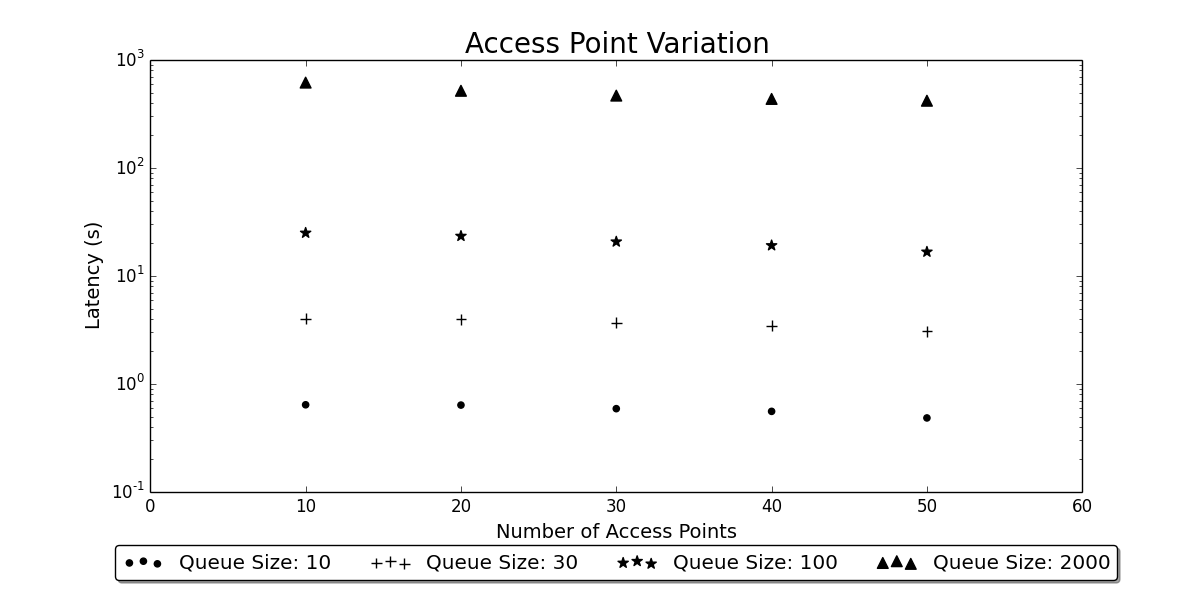
\includegraphics[width=\linewidth]{./images/Access_Point_Latency.png}
                \caption{}
                \label{fig:num_aps_latency}
            \end{subfigure}
            \begin{subfigure}{\textwidth}
                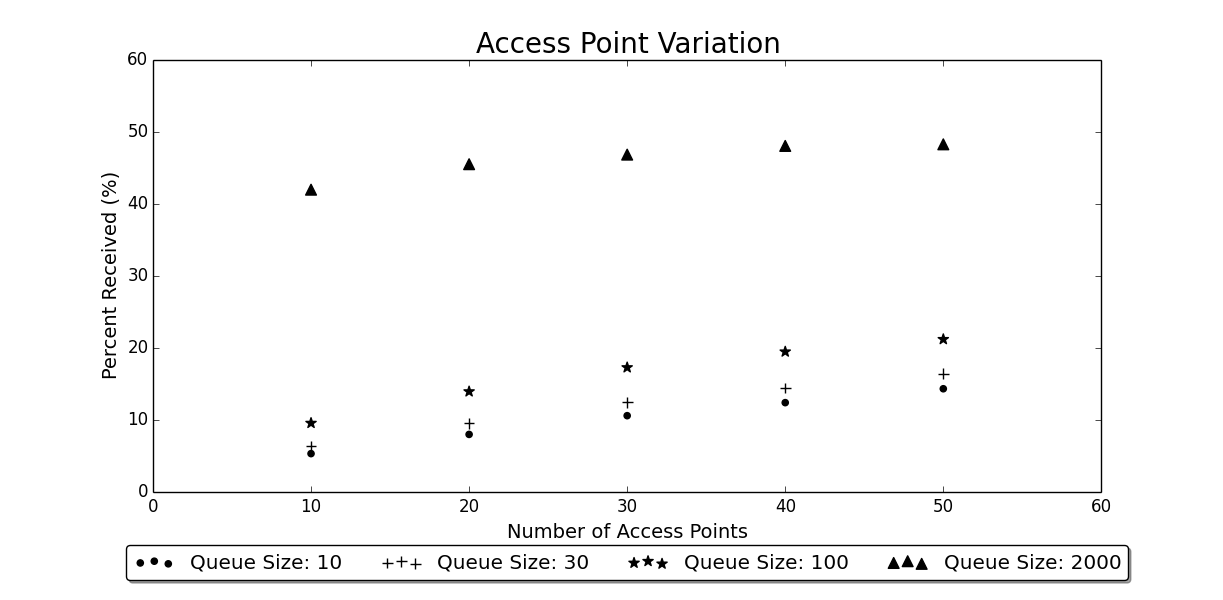
\includegraphics[width=\linewidth]{./images/Access_Point_Received.png}
                \caption{}
                \label{fig:num_aps_received}
            \end{subfigure}
            \caption{These figures show how the latency decreases with the number of access points (\ref{fig:num_aps_latency}), and the packet delivery rate increases (\ref{fig:num_aps_received}). (\ref{fig:num_aps_latency}) is plotted on a log scale in order to be able to differentiate between the various queue sizes.}
            \label{fig:num_aps}
        \end{figure}

        From this data we can see that the greater the number of access points the lower the latency and the greater the packet delivery rate. When adding a larger queue size the packet delivery rate increases but there is no improvement in latency, which manifests as a latency increase overall. With increasing the number of APs that disadvantage is no longer present. At smaller queue sizes we can double or even triple the packet delivery rate with more access points. It should be noted that as discussed in chapter~\ref{simulation} simulation time was one of the main factors for limiting the simulations to at most 50 access points. With the dataset we had over 2,000 access points. As such we can expect a much greater packet delivery rate with a significantly lower mean latency in an actual realisation of this model. 


    \section{Transmitter and Receiver Power}\label{data_gathering_performance_transmitter_and_reciever_power}

        A simple way of increasing the access point coverage of the city is to increase the power levels of the access points and receivers. This increase in power level causes them to serve a greater area without the need for any more access points. European legislation restricts all 2.4GHz radios to an equivalent isotropically radiated power level of 100mW~\cite{rackley2011wireless}. Converting to dBm gives a value of 19.93dBm, or approximately 20dBm. In practice we cannot increase the power levels of the radios without breaking the law, however we can do this with a simulator. In order to determine the effect that power level has on the data collection performance we tested the model at 5 different power levels. These power levels were 18, 19, 20, 21 and 22 dBm, which corresponds to 64.00, 80.63, 101.59, 128.00 and 161.27 respectively. Furthermore, we also must acknowledge that this is in fact a simulation and therefore not identical to a physical implementation. As such we need to also acknowledge that the propagation model will not be perfect. In order to find the most realistic model for our simulation we tried using 2 different models for this test. These propagation models were the Rayleigh model and the Log Normal Shadowing model. The results of this test, using a queue size of 2000 and all 50 access points, are shown in table~\ref{tab:power_level} and figure~\ref{fig:power_level}. 

        \afterpage{%
            \clearpage% Flush earlier floats (otherwise order might not be correct)
            \begin{landscape}
                \begin{table}
                    \centering
                    \begin{tabularx}{\linewidth}{|X|X|X|X|X|X|X|X|X|}
                        \hline
                        \multicolumn{1}{|X|}{\centering Power} & 
                        \multicolumn{1}{|X|}{\centering Model} & 
                        \multicolumn{1}{|X|}{\centering Mean \\ Latency (s)} & 
                        \multicolumn{1}{|X|}{\centering Standard \\ Deviation (s)} & 
                        \multicolumn{1}{|X|}{\centering Packets \\ Generated} & 
                        \multicolumn{1}{|X|}{\centering Packets \\ Sent} & 
                        \multicolumn{1}{|X|}{\centering Packets \\ Received} & 
                        \multicolumn{1}{|X|}{\centering Packets \\ Dropped} & 
                        \multicolumn{1}{|X|}{\centering \% \\ Received} \\
                        \hline
                        18 & Rayleigh & 154.12 & 323.82 & 294,743.60 & 522,092.80 & 238,455.20 & 1,986.40 & 80.74 \\
                        18 & Log Normal Shadowing & 122.62 & 278.35 & 279,041.50 & 452,601.00 & 225,997.50 & 2,268.75 & 79.72 \\
                        19 & Rayleigh & 128.94 & 281.37 & 270,759.00 & 473,615.20 & 213,552.20 & 933.20 & 78.72 \\
                        19 & Log Normal Shadowing & 169.79 & 363.87 & 527,232.75 & 868,566.75 & 431,838.25 & 34,279.50 & 83.15 \\
                        20 & Rayleigh & 150.13 & 322.72 & 299,218.50 & 525,681.25 & 240,421.75 & 1,445.50 & 80.26 \\
                        20 & Log Normal Shadowing & 150.72 & 316.18 & 470,629.50 & 782,219.50 & 388,500.00 & 20,491.00 & 81.03 \\
                        21 & Rayleigh & 116.22 & 255.51 & 220,911.00 & 383,434.50 & 169,469.00 & 0.00 & 76.79 \\
                        21 & Log Normal Shadowing & 86.43 & 203.14 & 179,300.00 & 290,371.00 & 134,968.00 & 0.00 & 75.27 \\
                        22 & Rayleigh & 135.75 & 294.37 & 270,957.00 & 471,525.67 & 218,749.33 & 977.33 & 80.54 \\
                        22 & Log Normal Shadowing & 0 & 0 & 0 & 0 & 0 & 0 & 0 \\
                        \hline
                    \end{tabularx}
                    \caption{The results of changing the power level of the radios.}
                    \label{tab:power_level}
                \end{table}
            \end{landscape}
        }

        \centerimagewide{./images/Power_Level.png}{A chart showing the small variations in latency and packet delivery when changing power level.}{fig:power_level}

        In terms of the propagation model a significant problem was found which may be apparent from the final row in table~\ref{tab:power_level}. There appeared to be a bug in the implementation in Omnet++ in which the simulation tended to crash when used with this simulation after some indeterminable period of time. Generally we did not get a simulation time of longer than 2,000 seconds which is significantly shorter than the 10,000 seconds we had been using previously. In some cases we did not get readings for particular runs using the Log Normal Shadowing model and therefore the mean result was made up of just 3 or 4 readings instead of 5. Furthermore, the effect that the software bugs had on the simulation when also trying the Log Normal Shadowing model also seemed to affect the simulation when going using the Rayleigh model, which is the model used for all other experiments. As such no further experiments were performed on propagation models. 

        With the results we have we can still analyse the effect that power level has. The effect is almost non-existent. We would expect to see a decrease in latency and increase in packet delivery as the power level goes up, however we saw no such increase. It is theorised that the reason for this is that the packet upload time is dominated by the bandwidth of the connection. By increasing the power levels we may be in contact with an access point for an extra few seconds, however as we can upload 2000 packets in less than a second, which is an effective rate of 48Kbps, this extra time only limits the delivery time of a single packet or two. Over a greater period of time, should the simulation have not crashed, it is possible that we may have seen a very small correlation, however it is insignificant at this time. 


    \section{Opportunistic Forwarding}\label{data_gathering_performance_opportunistic_forwarding}

        Opportunistic forwarding is the most significant change to the model that we will attempt. The implementation details are discussed in section~\ref{simulation_opportunistic_forwarding}. With the implementation discussed, the only way to evaluate the performance is to run a simulation both with and without opportunistic forwarding. The results of this are shown in tables~\ref{tab:opportunistic_forwarding_first} and \ref{tab:opportunistic_forwarding} and figure~\ref{fig:opportunistic_forwarding}.

        \afterpage{%
            \clearpage% Flush earlier floats (otherwise order might not be correct)
            \begin{landscape}
                \begin{table}
                    \centering
                    \begin{tabularx}{\linewidth}{|X|X|X|X|X|X|X|X|X|X|X|}
                        \hline
                        \multicolumn{1}{|X|}{\centering Queue Size} & 
                        \multicolumn{1}{|X|}{\centering Mean Latency (s)} & 
                        \multicolumn{1}{|X|}{\centering Standard Deviation} & 
                        \multicolumn{1}{|X|}{\centering AP Received} & 
                        \multicolumn{1}{|X|}{\centering AP Unique} & 
                        \multicolumn{1}{|X|}{\centering Packets Sent} & 
                        \multicolumn{1}{|X|}{\centering Packets Successful} & 
                        \multicolumn{1}{|X|}{\centering Packets Stored} & 
                        \multicolumn{1}{|X|}{\centering Packets Dropped} \\
                        \hline
                        10 & 0.23 & 1.39 & 463,908 & 421,622 & 2,160,545 & 463,239 & 57,673 & 833,967 \\
                        30 & 1.52 & 5.96 & 626,482 & 499,921 & 2,200,064 & 598,384 & 128,859 & 759,144 \\
                        100 & 12.02 & 30.38 & 829,123 & 513,153 & 2,490,028 & 733,816 & 341,718 & 753,631 \\
                        1000 & 236.26 & 370.09 & 1,475,528 & 659,686 & 4,063,488 & 1,121,781 & 1,827,617 & 438,549 \\
                        2000 & 344.52 & 633.09 & 1,534,024 & 648,545 & 4,825,887 & 1,109,934 & 2,605,998 & 289,271 \\
                        \hline
                    \end{tabularx}
                \end{table}
                \begin{table}
                    \centering
                    \begin{tabularx}{\linewidth}{|X|X|X|X|X|X|X|X|X|X|X|}
                        \hline
                        \multicolumn{1}{|X|}{\centering Queue Size} & \multicolumn{1}{|X|}{\centering AP Received} & \multicolumn{1}{|X|}{\centering AP Unique} & \multicolumn{1}{|X|}{\centering Packets Sent} & \multicolumn{1}{|X|}{\centering Packets Successful} & \multicolumn{1}{|X|}{\centering Packets Stored} & \multicolumn{1}{|X|}{\centering Packets Dropped} & \multicolumn{1}{|X|}{\centering Queue Ignores Time} & \multicolumn{1}{|X|}{\centering Queue Ignores Space} & \multicolumn{1}{|X|}{\centering Queue Ignores Ratio} & \multicolumn{1}{|X|}{\centering \% Received} \\
                        \hline
                        10 & 463,908 & 421,623 & 2,160,545 & 463,239 & 57,673 & 833,967 & 8,183,045 & 8,567,042 & 0.955 & 33.73\% \\
                        30 & 626,482 & 499,921 & 2,200,064 & 598,384 & 128,859 & 759,144 & 7,126,313 & 7,348,423 & 0.975 & 39.99\% \\
                        100 & 829,123 & 513,153 & 2,490,028 & 733,816 & 341,718 & 753,631 & 8,189,153 & 8,429,989 & 0.971 & 41.05\% \\
                        1000 & 1,475,528 & 659,686 & 4,063,488 & 1,121,781 & 1,827,617 & 438,549 & 6,906,153 & 6,976,392 & 0.990 & 52.77\% \\
                        2000 & 1,534,025 & 648,545 & 4,825,887 & 1,109,934 & 2,605,998 & 289,271 & 5,808,998 & 5,644,930 & 1.030 & 51.88\% \\
                        \hline
                    \end{tabularx}
                    \caption{These two tables are part of the same table, split across the page. They show the results of using opportunistic forwarding.}
                    \label{tab:opportunistic_forwarding_first}
                    \begin{tabularx}{0.6\linewidth}{|X|X|X|X|X|}
                        \hline
                        \multicolumn{1}{|X|}{\centering Queue Size} & 
                        \multicolumn{1}{|X|}{\centering Non OF Latency (s)} & 
                        \multicolumn{1}{|X|}{\centering OF Latency (s)} & 
                        \multicolumn{1}{|X|}{\centering Non OF \% Received} & 
                        \multicolumn{1}{|X|}{\centering OF \% Received} \\
                        \hline
                        10 & 0.49 & 0.23 & 14.34 & 33.73 \\
                        30 & 3.08 & 1.52 & 16.43 & 39.99 \\
                        100 & 16.72 & 12.02 & 21.21 & 41.05 \\
                        1000 & - & 236.26 & - & 52.77 \\
                        2000 & 419.84 & 344.52 & 48.29 & 51.88 \\
                        \hline
                    \end{tabularx}
                    \caption{This table shows the packet delivery ratio of using opportunistic forwarding versus not using opportunistic forwarding.}
                    \label{tab:opportunistic_forwarding}
                \end{table}
            \end{landscape}
        }

        \begin{figure}
            \centering
            \begin{subfigure}{\textwidth}
                \centering
                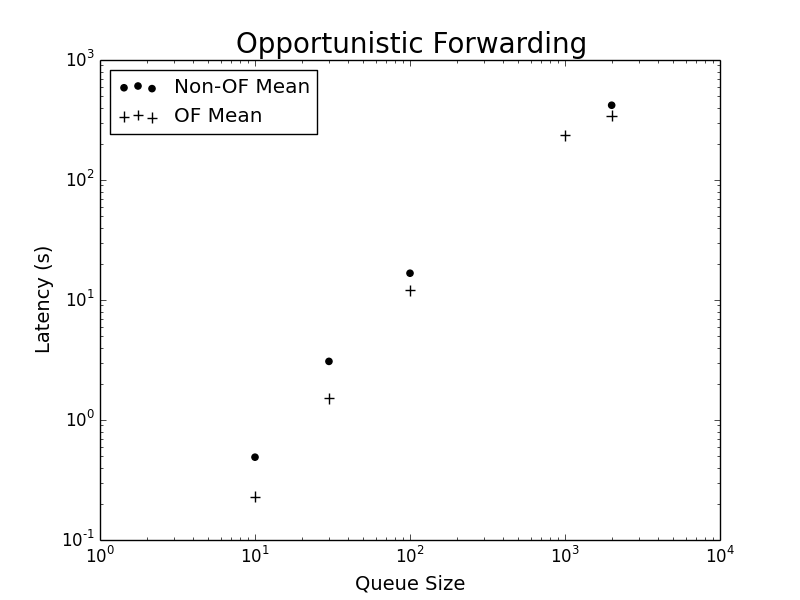
\includegraphics[width=\linewidth]{./images/OF_Latency.png}
                \caption{}
                \label{fig:of_latency}
            \end{subfigure}
            \begin{subfigure}{\textwidth}
                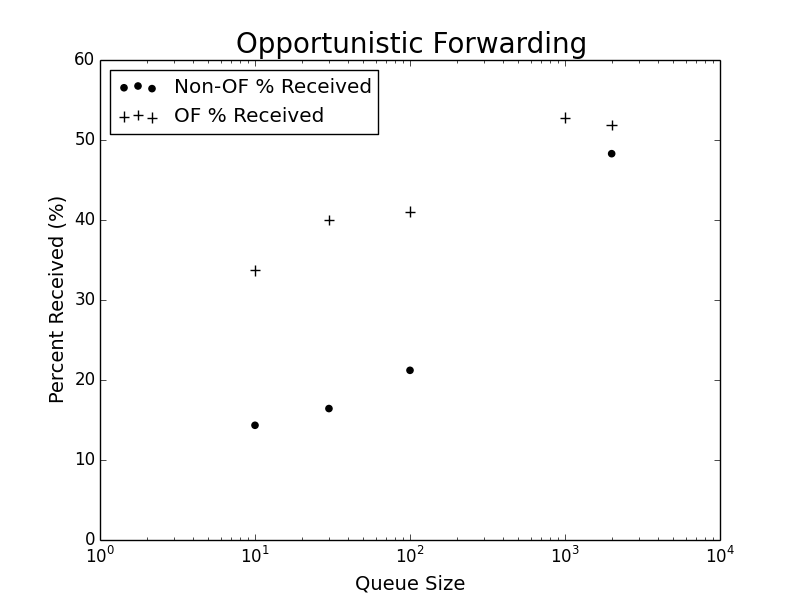
\includegraphics[width=\linewidth]{./images/OF_Received.png}
                \caption{}
                \label{fig:of_recieved}
            \end{subfigure}
            \caption{These figures show how the latency decreases when using opportunistic forwarding (OF) (\ref{fig:of_latency}), and the packet delivery rate increases (\ref{fig:of_latency}). Note that (\ref{fig:of_latency}) is on a log scale.}
            \label{fig:opportunistic_forwarding}
        \end{figure}

        With opportunistic forwarding, the same pattern is followed as with no opportunistic forwarding. When we increase the queue size, the packet delivery rate goes up, as does the latency. The interesting part is when we compare the two results. This is seen in table~\ref{tab:opportunistic_forwarding} and figure~\ref{fig:opportunistic_forwarding}. The results clearly show that using opportunistic forwarding increases the efficiency of our system. At low queue sizes, such as 10, it more than doubles the packet delivery ratio while also halving the mean latency. As we move to larger queue sizes the effect becomes less pronounced. With a queue size of 2000 we only increase the packet delivery rate from 48.29 to 51.88, however the average latency of a packet is over a minute less at just 344.5 seconds compared to 419.8 seconds. While the results seem to converge, it is unclear at this point if opportunistic forwarding would ever cause a detrimental effect to the results. 


    \section{Non-Chronological Queue}\label{data_gathering_performance_non-chronological_queue}

        Due to the apparent convergence of the results when using opportunistic forwarding a modification to the algorithm was proposed. In the initial runs, when bus $a$ received a packet from bus $b$ it would look at the time stamp on the packet from $b$ and use this to insert it into its own queue at the correct point. That is to say the queue of packets maintained by each bus is always in strict chronological order based on the packet generation time. In order to tell if any effects are caused because of this decision the same simulations as in section~\ref{data_gathering_performance_opportunistic_forwarding} were run once again, with the modification that any packets that $a$ receives from any other bus are simply placed at the end of the queue. The results of this compared to the original time stamp queued version are presented in table~\ref{tab:priority_queue} and figure~\ref{fig:priority_queue}.

        \begin{table}[H]
            \begin{tabularx}{\linewidth}{|X|X|X|X|X|}
                \hline
                \multicolumn{1}{|X|}{\centering Queue Size} & 
                \multicolumn{1}{|X|}{\centering Chronological Latency (s)} & 
                \multicolumn{1}{|X|}{\centering Non-Chronological Latency (s)} & 
                \multicolumn{1}{|X|}{\centering Chronological \% Received} & 
                \multicolumn{1}{|X|}{\centering Non-Chronological. \% Received} \\
                \hline
                10 & 0.23 & 0.20 & 33.73 & 37.71 \\
                30 & 1.52 & 1.00 & 39.99 & 38.67 \\
                100 & 12.02 & 6.98 & 41.05 & 42.75 \\
                1000 & 236.26 & 184.07 & 52.77 & 58.86 \\
                2000 & 244.52 & 373.48 & 51.88 & 65.60 \\
                \hline
            \end{tabularx}
            \caption{This table shows the packet delivery ratio of using opportunistic forwarding with the original queue based on time stamp  and the non-chronological version which appends all received packets to the queue.}
            \label{tab:priority_queue}
        \end{table}

        \begin{figure}
            \centering
            \begin{subfigure}{\textwidth}
                \centering
                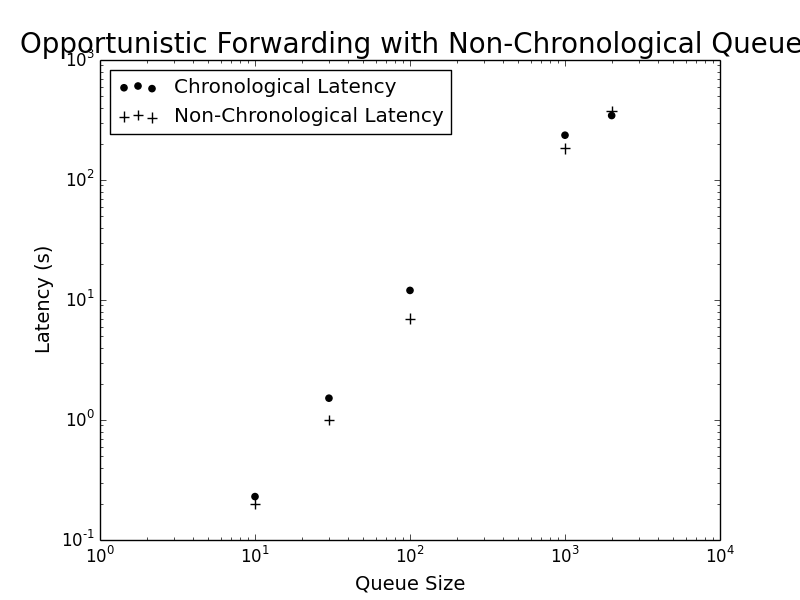
\includegraphics[width=\linewidth]{./images/OF_Non_Chron_Latency.png}
                \caption{}
                \label{fig:of_non_chron_latency}
            \end{subfigure}
            \begin{subfigure}{\textwidth}
                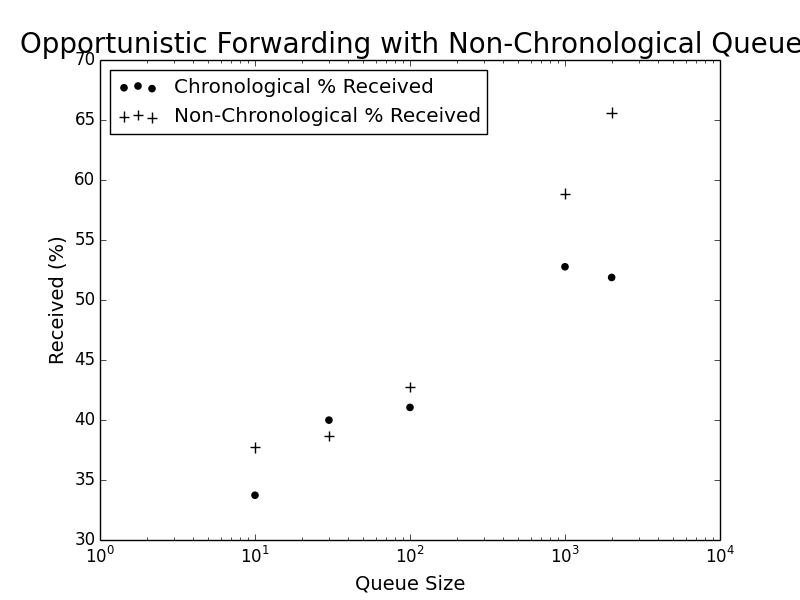
\includegraphics[width=\linewidth]{./images/OF_Non_Chron_Received.png}
                \caption{}
                \label{fig:of_non_chron_recieved}
            \end{subfigure}
            \caption{These figures show how the latency decreases when using a non-chronological queue with opportunistic forwarding (OF) (\ref{fig:of_non_chron_latency}), and the packet delivery rate increases (\ref{fig:of_non_chron_latency}). Note that (\ref{fig:of_non_chron_latency}) is on a log scale.}
            \label{fig:priority_queue}
        \end{figure}

        The results from this show that at smaller queue sizes, that is 10-1000 packets, the latency is even lower when simply appending to the end of the queue. At all measured queue sizes, with the exception of 30 which could simply be a statistical anomaly, the packet delivery rate is significantly improved. However, at higher queue sizes, 2000 onwards, it seems that this advantage is diminished by the increased latency. This is however expected. As we have discussed in previous sections, the price paid for holding onto more packets for longer in order to ensure they are delivered, is that the latency will increase. 

        The unexpected effect is that appending to the end of the queue instead of inserting into the correct position has a positive effect on the delivery ratio. We would expect this to have no change at all. This effect is due to duplication of packets. If a bus, $a$, broadcasts a packet and there are 4 buses in the immediate vicinity who accept the packet then we have 4 duplicates. $a$ will receive a response and then move on to broadcasting the next packet in the queue, ignoring that 4 buses have the packet now. When a bus gets a full queue from a miscalculation of when it will encounter an access point it drops the packets at the front of the queue. In the priority queue version where we insert packets at the correct position, the oldest packets are penalised and since the duplicates all have the same time stamp they will tend to all be dropped, rather than the unique packets that the buses carry. 

        When we compare this result to the base line, as in table~\ref{tab:opportunistic_queue_good} and figure~\ref{fig:opportunistic_queue_good}, without opportunistic forwarding, the results are striking. With a queue size of 10 we get 163\% and 145\% better performance in terms of packet delivery and latency respectively. With the largest queue size of 2,000 we get an increase of 37\% and 12\% in terms of packet delivery and latency respectively. Again, it seems like these two series will converge, but not until we reach 100\% packet delivery.

        \begin{table}
            \centering
            \begin{tabularx}{0.8\linewidth}{|X|X|X|X|X|}
                \hline
                \multicolumn{1}{|X|}{\centering Queue Size} & 
                \multicolumn{1}{|X|}{\centering Non OF Latency (s)} & 
                \multicolumn{1}{|X|}{\centering OF Latency (s)} & 
                \multicolumn{1}{|X|}{\centering Non OF \% Received} & 
                \multicolumn{1}{|X|}{\centering OF \% Received} \\
                \hline
                10 & 0.49 & 0.20 & 14.34 & 37.71 \\
                30 & 3.08 & 1.00 & 16.43 & 38.67 \\
                100 & 16.72 & 6.98 & 21.21 & 42.75 \\
                1000 & - & 184.07 & - & 58.86 \\
                2000 & 419.84 & 373.48 & 48.29 & 65.60 \\
                \hline
            \end{tabularx}
            \caption{This table shows the packet delivery ratio of using opportunistic forwarding versus not using opportunistic forwarding.}
            \label{tab:opportunistic_forwarding}
        \end{table}
        
        \begin{figure}
            \centering
            \begin{subfigure}{\textwidth}
                \centering
                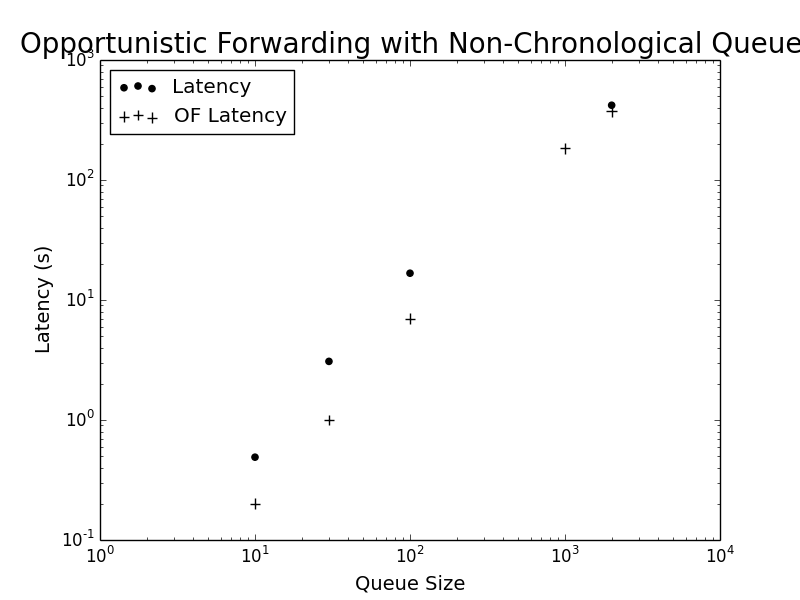
\includegraphics[width=\linewidth]{./images/OF_Complete_Latency.png}
                \caption{}
                \label{fig:of_complete_latency}
            \end{subfigure}
            \begin{subfigure}{\textwidth}
                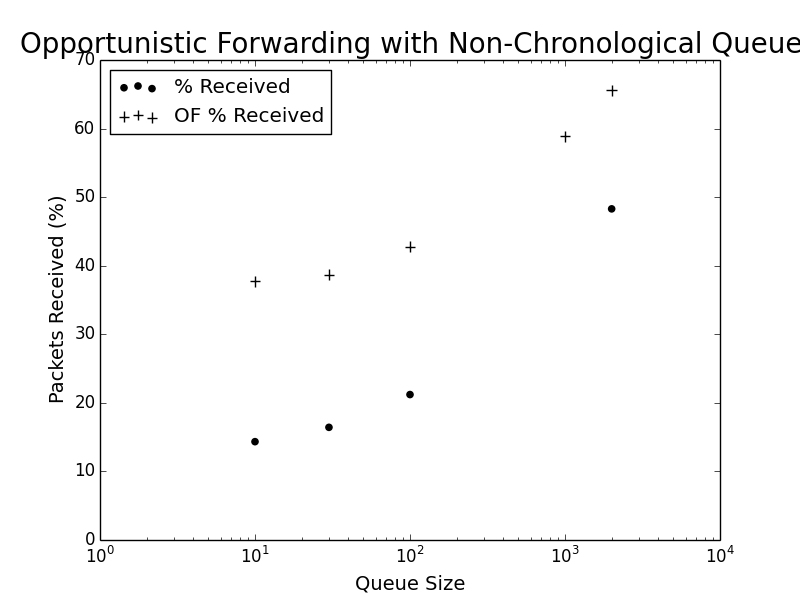
\includegraphics[width=\linewidth]{./images/OF_Complete_Received.png}
                \caption{}
                \label{fig:of_complete_recieved}
            \end{subfigure}
            \caption{These figures compare opportunistic forwarding with a non-chronological queue against the results of simulations where opportunistic forwarding is not used. They show how the latency decreases when using opportunistic forwarding (OF) (\ref{fig:of_complete_latency}), and the packet delivery rate increases (\ref{fig:op_complete_received}). Note that (\ref{fig:of_complete_latency}) is on a log scale.}
            \label{fig:opportunistic_queue_good}
        \end{figure}

    \section{Conclusions}\label{data_gathering_performance_conclusions}

        \tdi{Probably rewrite this conclusion from scratch. It is awful. I need to cover what optimisations were best, how much they improved things by and whether this system is of any use to Edinburgh.}

        Some of the information we have learned from the simulation is expected, such as increasing the number of access points increases packet delivery and reduces latency, however some of it is unexpected. Increasing the queue size causing an increase in latency was not an obvious result before hand, however it has made it clear that there is a trade off between packet delivery rates and packet latency. Perhaps surprisingly transmitter power had almost no effect on the results due to the connection speed dominating the small increase in distance. 

        The most effective optimisation was the introduction of opportunistic forwarding. When using the non-deterministic version of the queuing mechanism the results are extremely promising. In practice, we have many more access points within the city and from these results it is reasonable to estimate that in practice our packet delivery rate could be over 90\%. 

        Due to using a simulation rather than real world tests it can be difficult to confirm that in reality we would get such good results. Unfortunately we almost definitely not see such good results. This simulation treats Edinburgh as a two dimensional map. There is no concept of terrain and buildings. The simulation assumes that there is line of sight between the sensors and the access points, however this is unlikely to always be the case. These access points will be in buildings, which has already partially been taken into account with the simulation as we had information about relative signal strength, and may be blocked by other structures. We know that in a physical implementation of this model we would spend less time in contact with access points than we currently do, and most likely be in contact with a smaller number of access points. It is important to remember that we have the data for over 2,000 access points around the city, not just the 50 that we can simulate at a time. If we only manage to contact half the access points that we manage in this simulation, then we have 1,000 useful access points across the city. This is twenty times the number of access points we use in the simulation. The results from this chapter are very encouraging, and show that implementing such a model in Edinburgh would be effective. 

